% !TeX spellcheck = de_DE
\chapter{ANSA}
Når mamma og pappa er 5400 km unna...
Alle som studerer utenlands vil støte på store eller små problemer underveis. Noen problemer løses lett ved en telefon hjem til mor og far. Husk at også vi er her for deg mens du er ute i verden og studerer. \\
\url{http://www.ansa.no}


\section{Hva kan ANSA hjelpe deg med?}
Du kan bli medlem av ANSA når du har fått en studieplass i utlandet. Som medlem kan du tegne ANSA Studentforsikring og ANSA Pluss og du kan delta på våre arrangementer i Norge og utlandet. Du får også rådgivning hvis du får problemer under studieoppholdet, tilsendt medlemsbladet ANSAnytt i posten og jobbtilbud på e-post.
Trenger du bistand i forhold til problemer i studielandet eller informasjon om forhold og instanser i Norge, kan du ta kontakt med ANSAs rådgivere. Kontakt rådgiverne per e-post eller per telefon 22 47 76 00.


\begin{figure}[h]
\center
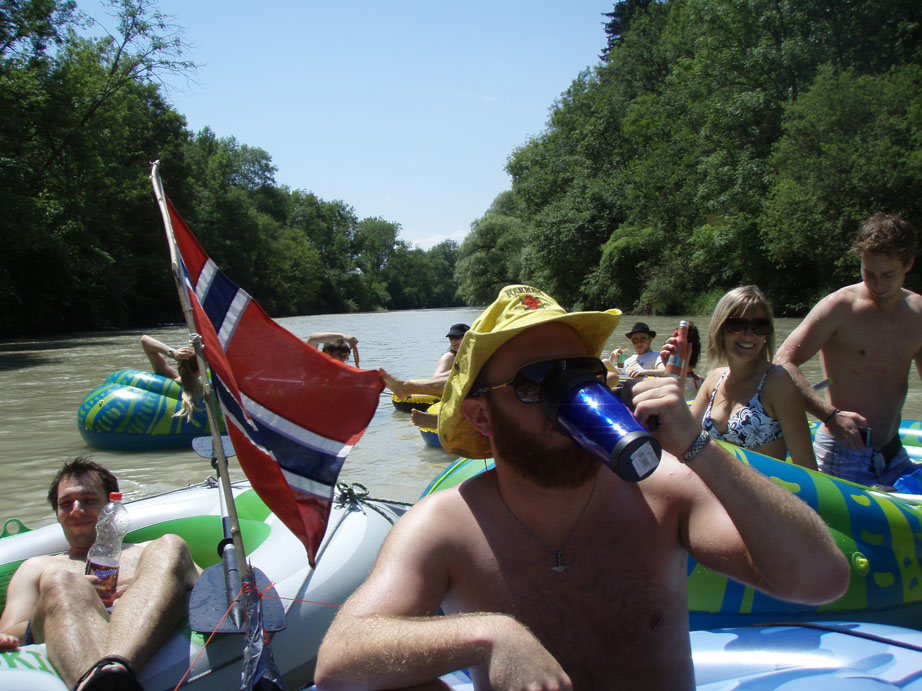
\includegraphics[width=0.31\textwidth]{./gfx/isar}
\caption{Tørste sjørøvere på tokt i Isar}
\end{figure}





\section{ANSA München}
Vi er omlag 12 heltidsstudenter og langt flere utvekslingsstudenter. De fleste har god kontakt med hverandre. De fleste studerer medisin, i tillegg er det noen som studerer informatikk, matematikk eller andre ingeniørfag.

Hvert år arrangerer vi 16. mai - russefest, juletrefest og felles turer. Det Norske Konsulatet står for 17. mai, og svenskene treffer vi på St. Hans.
ANSA arrangerer semester-kickoff hver semesterstart, og treffes jevnlig i semesteret. Det er et par sentrale norske personer (ikke bare ANSA-medlemmer) som organiserer disse jevnlige "Stammtischene". Informasjon om dette finner en i vår facebookgruppe "Norwegischer Stammtisch München / ANSA München". Her opplyses det altså om de vanlige "Stammtischene" og ANSA-arrangerte events. Her blir alle som vil komme; venner, kjente og norsk-interesserte invitert. Hvis det er noe som er kun ment for ANSA-medlemmer, går dette over e-mail.\\
\url{http://www.ansa.no/ANSAland/Tyskland/Lokallag/ANSA-Munchen/}

Facebook:\\
\url{http://www.facebook.com/groups/2244635897}

\section{Russefest}

bla bla

\section{17. Mai}
\begin{figure}[h]
\center

\includegraphics[width=0.31\textwidth]{./gfx/17mai}
\caption{Nordmenn i tog ved Chinesischer Turm i Englischer Garten}
\end{figure}


\section{Juletrefest}


\section{Isar River-run}
bla bla hvert år,.. s-bahn osv.



\section{Norwegerfete}

blablabla




\section{Hva koster medlemskap i ANSA?}

\begin{enumerate}
\item Halvårsmedlemskap (vår/høst) koster 250,-.
\item Skoleårsmedlemskap (dvs. fra 1. juli til og med 31. juli året etter) og kalenderårsmedlemskap (dvs. fra og med 1. januar til og med 31. januar året etter) koster 375,-.
\item Tegner du medlemskap for flere år av gangen er prisen:
\begin{enumerate}
\item 2 år: kr. 645,- 
\item 3 år: kr. 865,-
\item 4 år: kr. 975,-
\item 5 år: kr. 1125,-
\item 6 år. kr. 1275,-
\end{enumerate}
\end{enumerate} 


\section{ANSA Forsikring}
Hva må til for at jeg kan tegne ANSA forsikring?
For å kunne tegne ANSA studentforsikring må du være medlem av ANSA, samt være medlem av norsk folketrygd, eller ha rett til utvidet stønad til helsetjenester NAV internasjonalt.

\subsection{Hva koster forsikringen?}
ANSA studentforsikring er delt inn i en Nordengrunnpakke, Europagrunnpakke og en Verdensgrunnpakke. I tillegg kan man tegne en valgfri sykeforsikring i tillegg til Europa- eller Verdensgrunnpakken. Forsikringen kan tegnes for enten 4, 6 eller 12. måneder. Prisinformasjon finner du på \url{www.ansa.no/forsikring}.

\subsection{Hva dekker forsikringen?}
ANSAs studentforsikring er spesialdesignet for utenlandsstudenter og består blant annet av innbo-, ulykke- og studieavbruddsforsikring, samt forsikring som dekker hjemkallelse og reisegods. I tillegg kan man tegne en valgfri sykeforsikring.

\section{Studentavis}
Norwegern er avisen for norske studenter i Tyskland. Den skal utgis to ganger i året, i begynnelsen av vintersemesteret, vanligvis på organisasjonskurset, og i begynnelsen av sommersemesteret, her blir den utgitt på landsmøtet.
Oppmøtte ved organisasjonskurset og landsmøtet tar med seg aviser og deler ut til medlemmene i sin by, ellers blir avisene sendt ut. Har du ikke fått avisen? Send en email til redaktøren, så blir det en ordning på det!
Avisen skal være selvforsørgende, dvs at utgiftene skal dekkes av reklame i avisen. Har din bedrift lyst til å støtte avisen og reklamere? Ta kontakt med markedsansvarlig her.
På denne siden vil du finne de siste utgavene av Norwegern og artikler fra eldre utgaver. God fornøyelse!

\begin{figure}[h]
\center
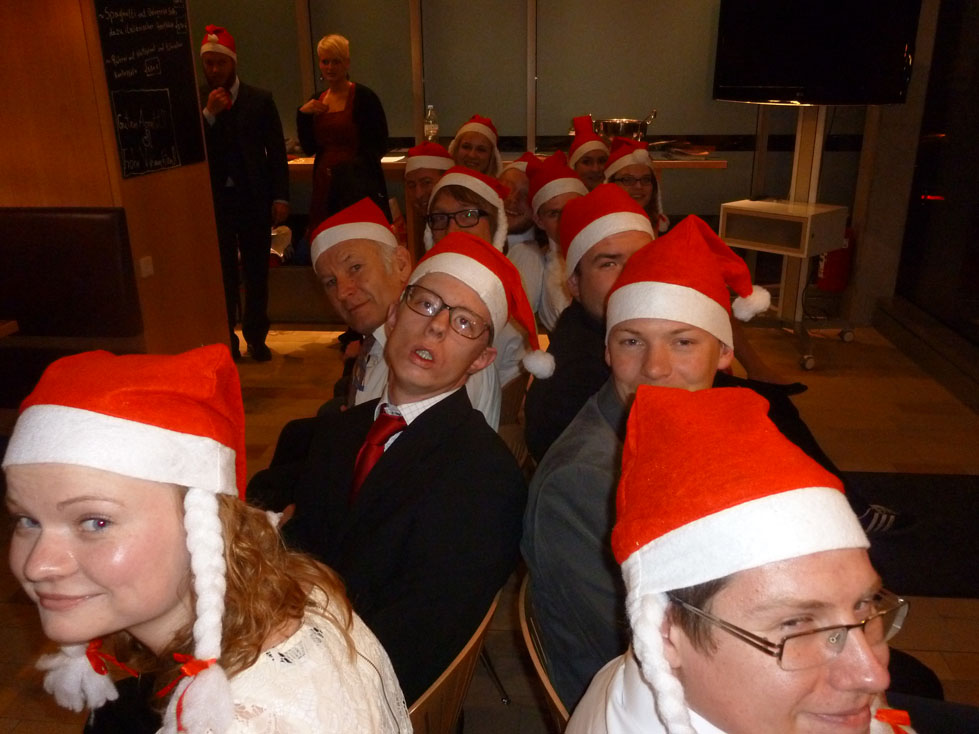
\includegraphics[width=0.31\textwidth]{./gfx/juletrefest}
\caption{Nisser klare for stolleken}
\end{figure}

\section{Sjømannskirken}
Sjømannskirkene og ANSA har utviklet en beredskapsplan for tilfeller der det skjer ulykker i utlandet. Beredskapen består for vår del av presidenten i ANSA, medlemsservice, infosenteret, rådgiverne og studentprestene, som jo hører under Sjømannskirken. Hvis du står ovenfor en ulykke eller en katastrofe av noe slag, gjør du klokt i å ringe enten presidenten eller studentpresten din. Disse vil ringe og kontakte de andre i beredskapsgruppa. De varsler også UD. Det neste de gjør er åsjekke om det finnes studenter hvor ulykken inntraff og kontakter disse. I tillegg diskuteres hva som bør gjøres og de avventer nærmere beskjeder.

\begin{figure}[h]
\center
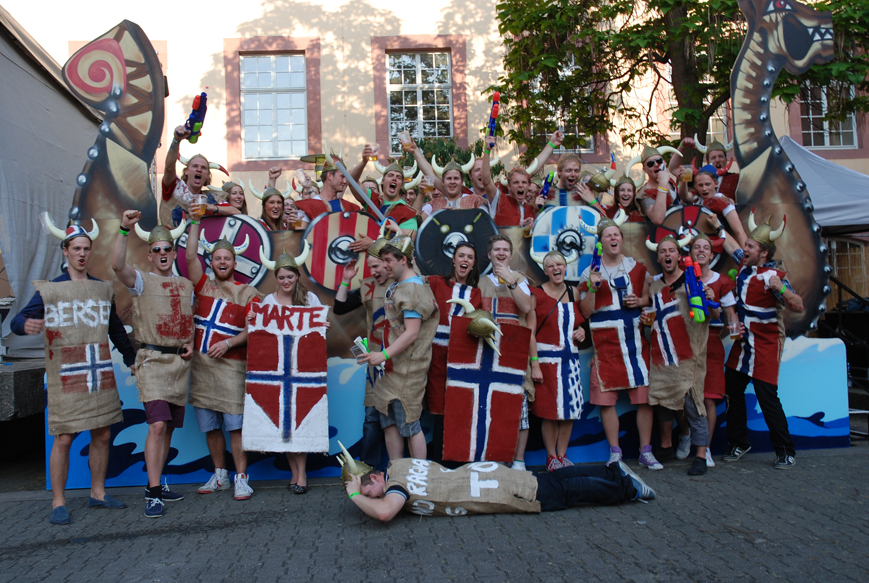
\includegraphics[width=0.31\textwidth]{./gfx/norwegerfete}
\caption{Norwegerfete i Mannheim}
\end{figure}
